\documentclass{article}
\usepackage[a4paper, margin=3mm, landscape]{geometry}
\usepackage{multicol}
\usepackage{xcolor}
\usepackage{enumitem}
\usepackage{amsmath}
\usepackage{amsfonts}
\usepackage{listings}
\usepackage{soul}
\usepackage{graphicx}

\pdfinfo{
    /Title (MA2104.pdf)
    /Creator (TeX)
    /Producer (pdfTeX 1.40.0)
    /Author (Jason Qiu)
    /Subject (MA2104)
    /Keywords (MA2104, nus, cheatsheet, pdf)
}

\graphicspath{ {./img/} }

\pagestyle{empty}
\setcounter{secnumdepth}{0}
\setlength{\columnseprule}{0.25pt}

% Redefine section commands to use less space
\makeatletter
\renewcommand{\section}{\@startsection{section}{1}{0mm}%
    {-1ex plus -.5ex minus -.2ex}%
    {0.5ex plus .2ex}%x
{\normalfont\large\bfseries}}
\renewcommand{\subsection}{\@startsection{subsection}{2}{0mm}%
    {-1explus -.5ex minus -.2ex}%
    {0.5ex plus .2ex}%
{\normalfont\normalsize\bfseries}}
\renewcommand{\subsubsection}{\@startsection{subsubsection}{3}{0mm}%
    {-1ex plus -.5ex minus -.2ex}%
    {1ex plus .2ex}%
{\normalfont\small\bfseries}}%
\makeatother

% Adjust spacing for all itemize/enumerate
\setlength{\leftmargini}{0.5cm}
\setlength{\leftmarginii}{0.5cm}
\setlist[itemize,1]{leftmargin=2mm,labelindent=1mm,labelsep=1mm}
\setlist[itemize,2]{leftmargin=2mm,labelindent=1mm,labelsep=1mm,label=$\bullet$}

% Font
\renewcommand{\familydefault}{\sfdefault}

% Define colors for math formulas
\definecolor{myblue}{cmyk}{1,.72,0,.38}
\everymath\expandafter{\the\everymath \color{myblue}}

% Custom command for keywords
\definecolor{highlight}{RGB}{251,243,218}
\newcommand{\keyword}[2]{\sethlcolor{highlight}\hl{\textbf{#1}} - #2}
\newcommand{\ilkeyword}[1]{\sethlcolor{highlight}\hl{\textbf{#1}}}

% Custom command for partial derivatives
\newcommand{\partialderivative}[2][]{\frac{\partial #1}{\partial #2}}

% Define colors and style for code
\definecolor{codegreen}{rgb}{0,0.6,0}
\definecolor{codegray}{rgb}{0.5,0.5,0.5}
\definecolor{codered}{HTML}{CC241D}
\definecolor{backcolor}{rgb}{0.95,0.95,0.95}
\lstdefinestyle{codestyle}{
    backgroundcolor = \color{backcolor},
    commentstyle = \color{codegray},
    keywordstyle = \color{codered},
    stringstyle = \color{codegreen},
    basicstyle = \ttfamily,
    breakatwhitespace = false,
    showstringspaces = false,
    breaklines = true,
    showtabs = false,
    tabsize = 2
}
\lstset{style = codestyle}

% -----------------------------------------------------------------------
\begin{document}
\begin{multicols*}{4}
\footnotesize

% Title box
\begin{center}
    \fbox{
        \parbox{0.8\linewidth}{
            \centering \textcolor{black}{
                {\Large\textbf{MA2104}} \\
                \normalsize{AY23/24 Sem 2}} \\
                {\footnotesize \textcolor{gray}{github.com/jasonqiu212}}
        }
    }
\end{center}

\section{01. Vectors, Lines, Planes}

\begin{itemize}
    \item \keyword{Dot Product}{$a \cdot b = ||a||||b|| \cos \theta$}
    \begin{itemize}
        \item $a \cdot b = b \cdot a$ $\quad$ $a \cdot (b + c) = a \cdot b + a \cdot c$ 
        \item $a \cdot b = 0 \leftrightarrow a \perp b$
    \end{itemize}
    \item \keyword{Projection}{$\text{proj}_{a}b = \frac{a \cdot b}{a \cdot a} a$}
    \begin{itemize}
        \item $\text{comp}_{a} b = ||\text{proj}_{a}b|| = \frac{a \cdot b}{||a||}$
    \end{itemize}
    \item \keyword{Cross Product}{$a \times b =
        \begin{vmatrix}
            i & j & k \\ 
            a_1 & a_2 & a_3 \\ 
            b_1 & b_2 & b_3 \\ 
        \end{vmatrix} = \langle a_2 b_3 - a_3 b_2, -(a_1 b_3 - b_1 a_3), a_1 b_2 - a_2 b_1 \rangle$}
    \begin{itemize}
        \item $a \times b \perp a$ and $\perp b$ $\quad$ $a \times b = - b \times a$
        \item $||a \times b|| = ||a||||b|| \sin \theta$ $\quad$ Direction: Right hand rule
        \item $A = ||a \times b||$ $\quad$ $||PQ||\sin \theta = \frac{||PQ \times PR||}{||PR||}$
    \end{itemize}
\end{itemize}

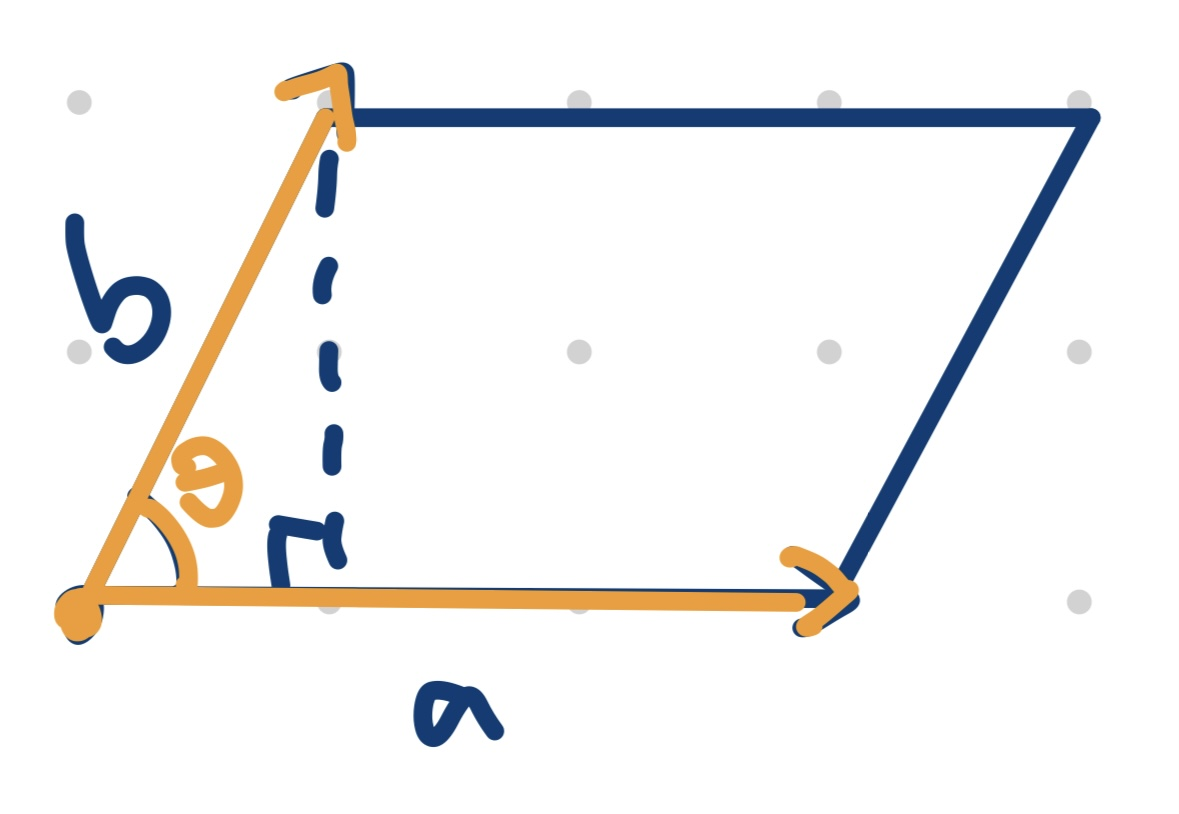
\includegraphics[scale=0.05]{area-of-parallelogram.jpg}
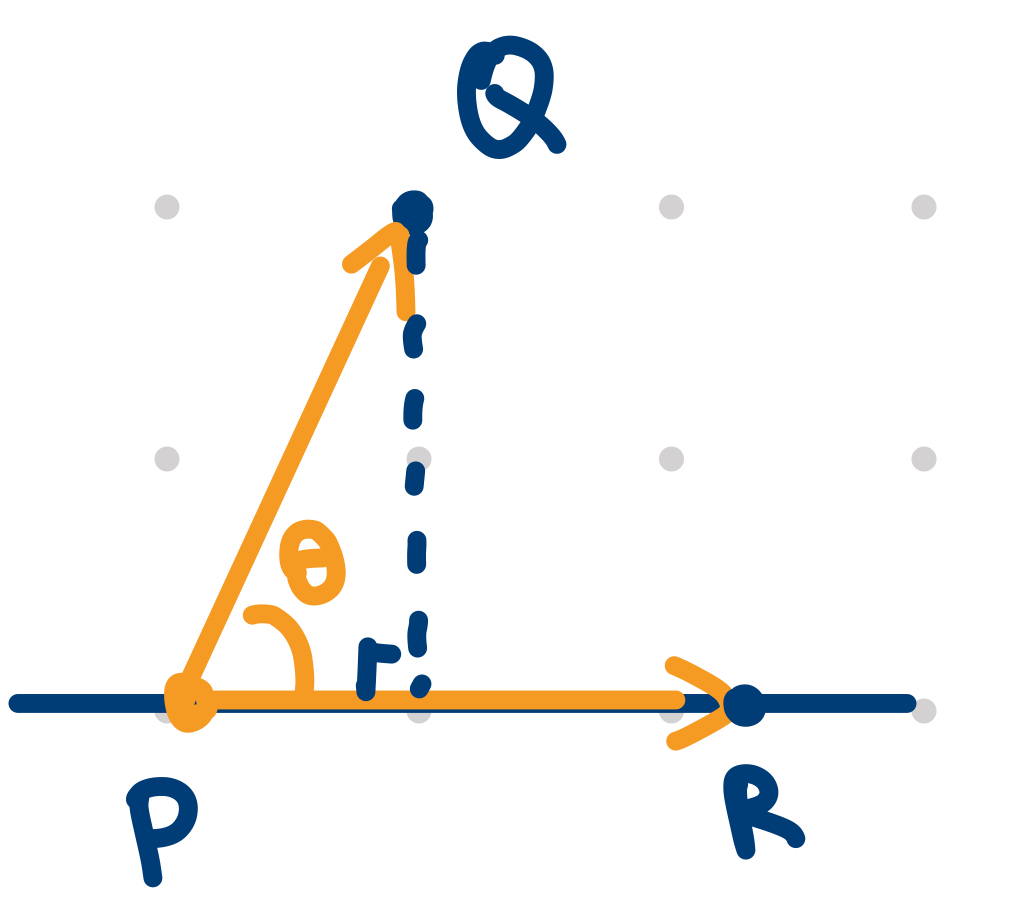
\includegraphics[scale=0.05]{distance-from-point-to-line.jpg}

\begin{itemize}
    \item \keyword{Scalar Triple Product}{$a \cdot (b \times c) = 
    \begin{vmatrix}
        a_1 & a_2 & a_3 \\ 
        b_1 & b_2 & b_3 \\ 
        c_1 & c_2 & c_3 \\ 
    \end{vmatrix}$}
    \begin{itemize}
        \item Result is a scalar value
        \item $A_{\text{Base}} = ||b \times c||$ $\quad$ $V = Ah = a \cdot (b \times c)$
    \end{itemize}
\end{itemize}

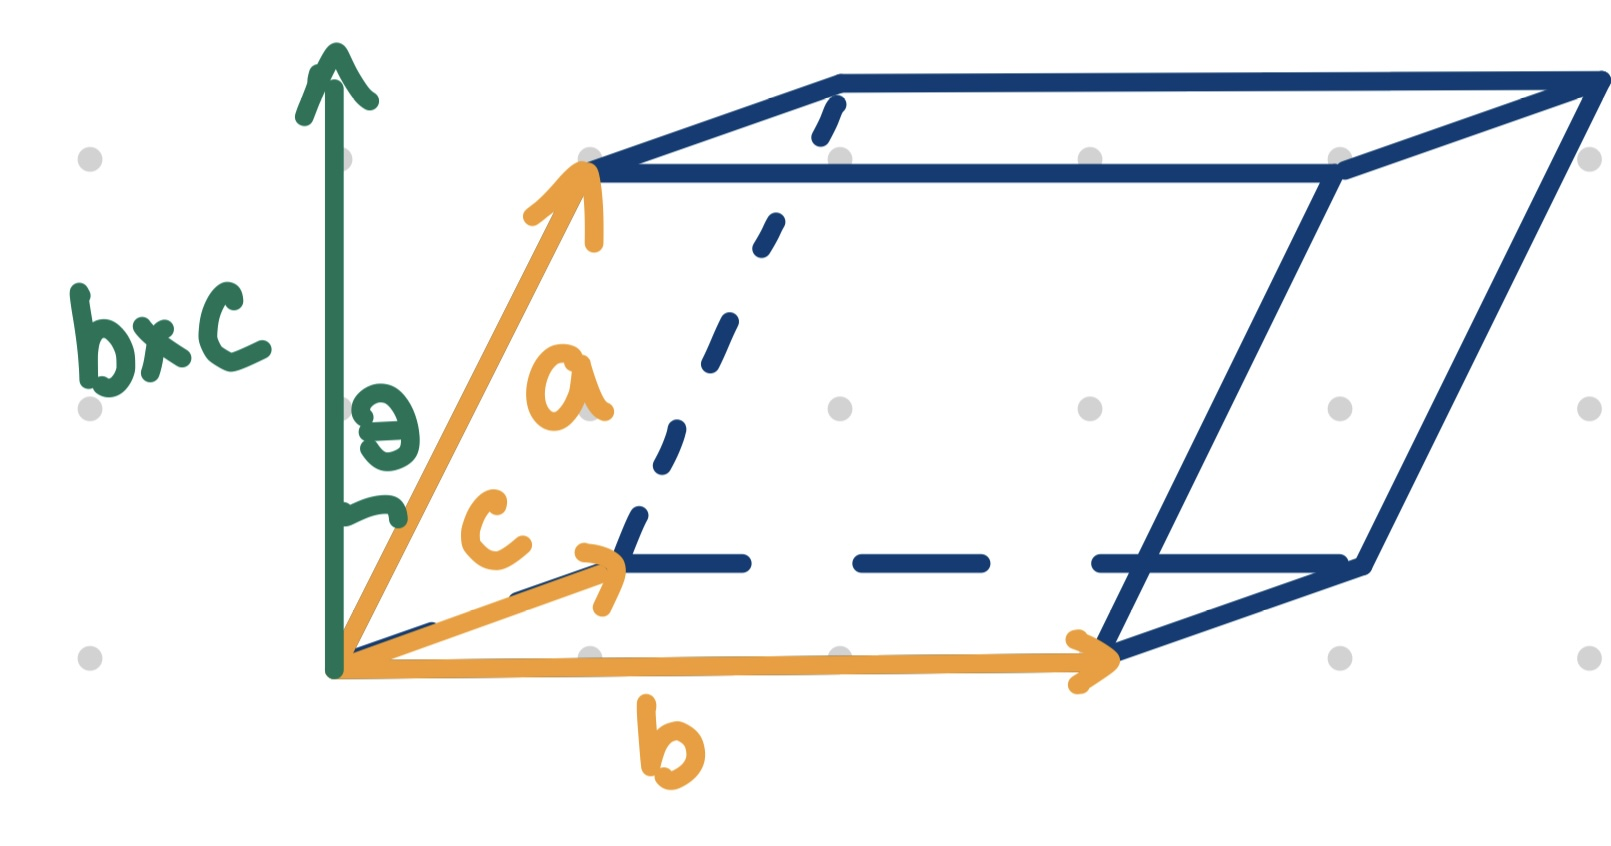
\includegraphics[scale=0.05]{volume-of-parallelepiped.jpg}

\begin{itemize}
    \item \keyword{Line}{$\langle x, y, z \rangle = \langle x_0, y_0, z_0 \rangle + \langle a, b, c \rangle t$}
    \begin{itemize}
        \item 2D: Either parallel or intersecting
        \item 3D: Either parallel, intersecting, or skew
    \end{itemize}
    \item \keyword{Plane}{$\langle a,b,c \rangle \cdot \langle x,y,z \rangle = \langle a,b,c \rangle \cdot \langle x_0,y_0,z_0 \rangle$ where $\langle a,b,c \rangle$ is perpendicular to plane}
    \item \keyword{Tangent Vector}{Given $r(t) = \langle f(t),g(t),h(t) \rangle$:}
\end{itemize}

\[
    r'(a) = \lim_{\triangle{t} \rightarrow 0} \frac{r(a + \triangle{t}) - r(a)}{\triangle{t}} = \langle f'(a),g'(a),h'(a) \rangle
\]
\begin{itemize}
    \item $\frac{d}{dt}(r(t) + s(t)) = r'(t) + s'(t)$
    \item $\frac{d}{dt}(r(t)s(t)) = r'(t)s(t)+r(t)s'(t)$
    \item $\frac{d}{dt}(r(t) \cdot s(t)) = r'(t) \cdot s(t)+r(t) \cdot s'(t)$
    \item $\frac{d}{dt}(r(t) \times s(t)) = r'(t) \times s(t)+r(t) \times s'(t)$
    \item \keyword{Arc Length}{Given smooth $r(t) = \langle f(t),g(t),h(t) \rangle$:}
\end{itemize}

\[
    S = \int_{a}^{b} ||r'(t)|| dt
\]

\section{02. Functions of 2 Variables}

\begin{itemize}
    \item \keyword{Surface}{$z = f(x,y)$}
    \item \keyword{Horizontal Trace}{(Level curve) Intersects with horizontal plane (i.e. $f(x,y) = k$)}
    \begin{itemize}
        \item \keyword{Level Surface}{$f(x,y,z) = k$}
    \end{itemize}
    \item \keyword{Vertical Trace}{Intersections with vertical plane}
    \item \keyword{Contour Plot}{$f(x,y) = k$ with lots of $k$'s}
    \item \keyword{Quadric Surfaces}{$Ax^2+By^2+Cz^2+J = 0$ or $Ax^2+By^2+Iz=0$}
    \begin{itemize}
        \item \keyword{Cylinder}{There exists plane such that all planes parallel to plane intersect surface in some curve}
    \end{itemize}
\end{itemize}
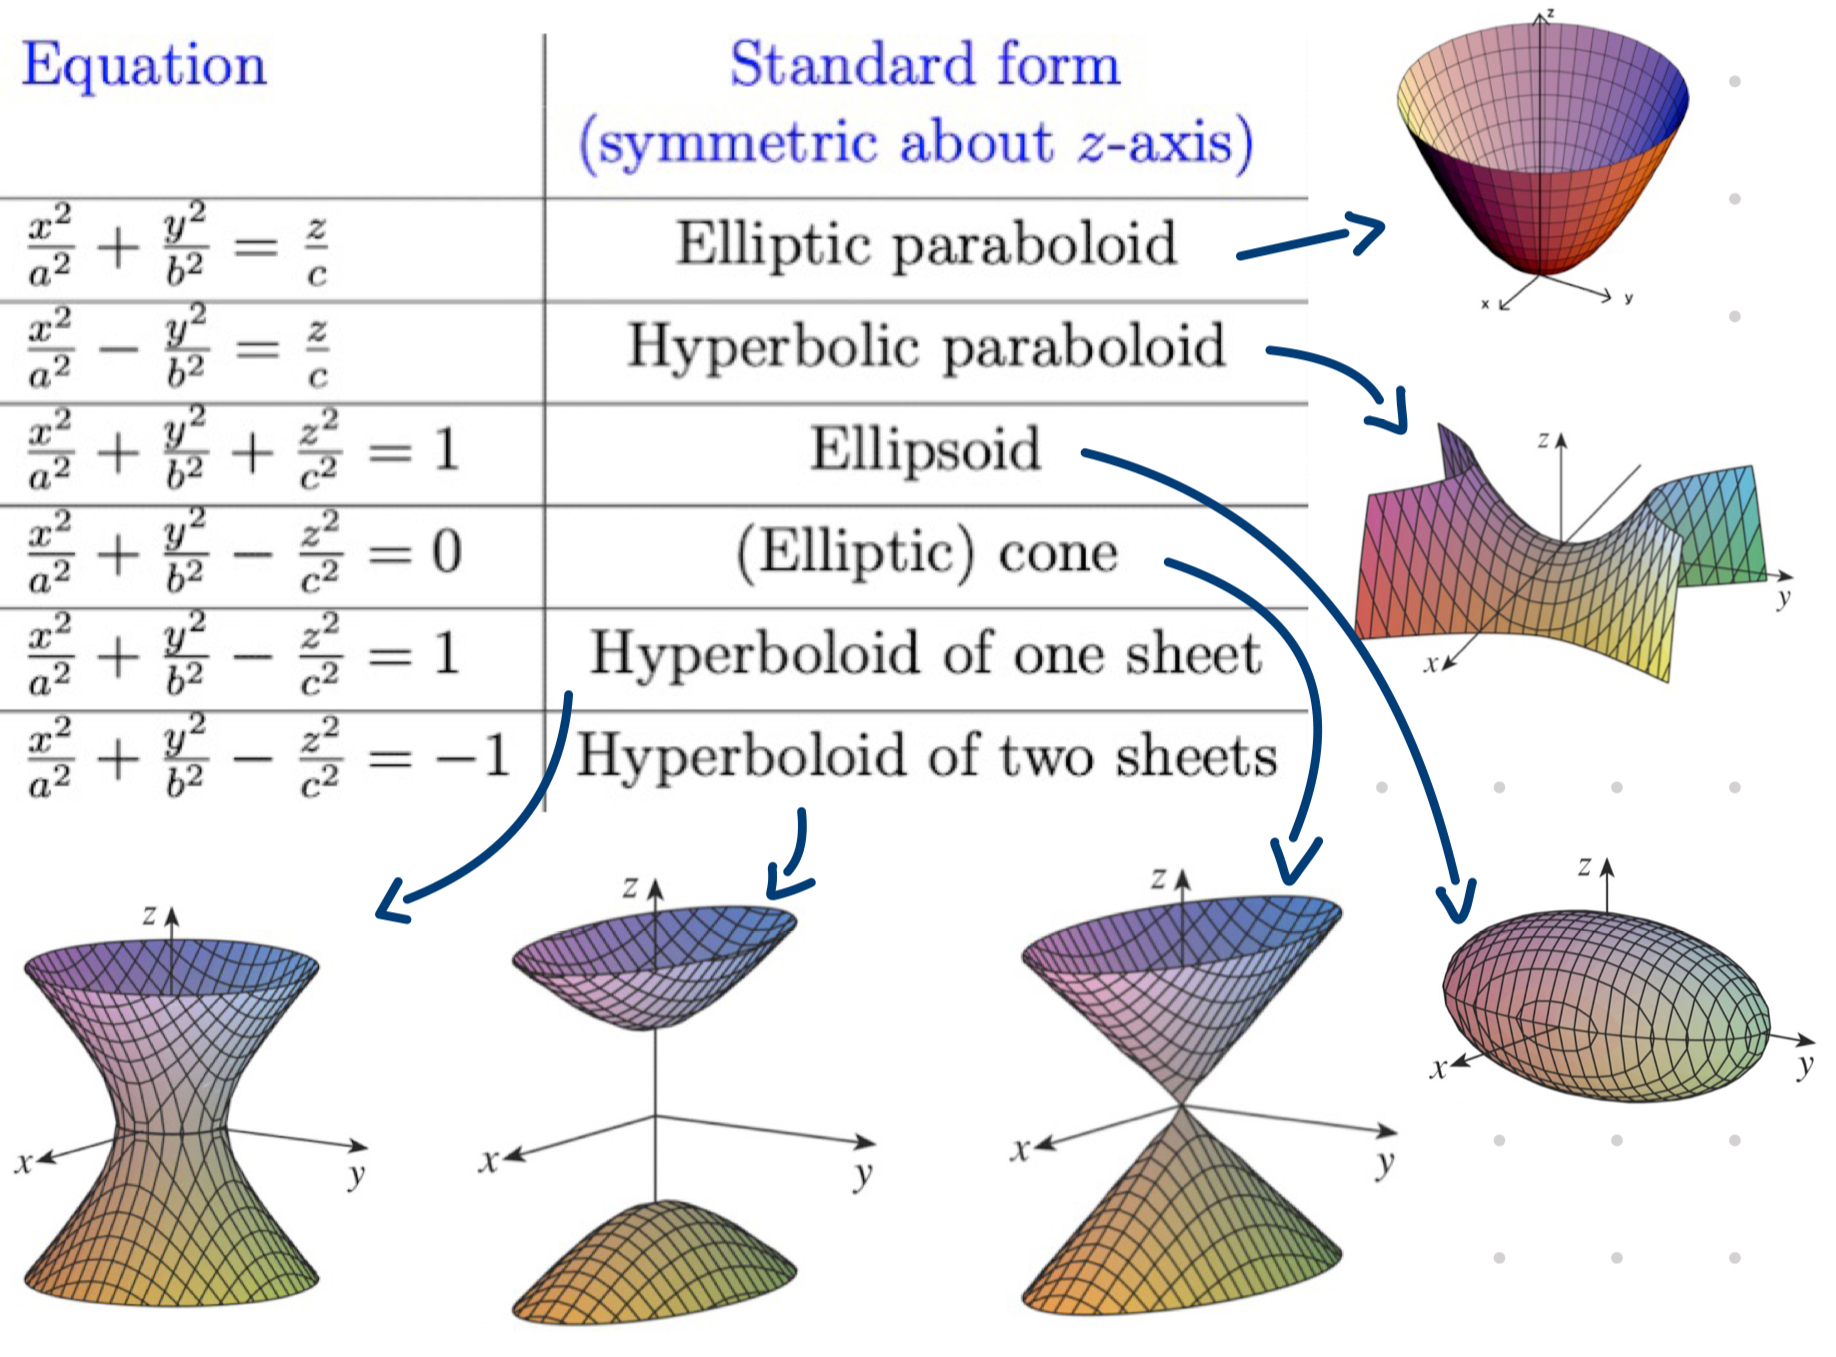
\includegraphics[scale=0.097]{quadric-surfaces.jpg}

\begin{itemize}
    \item \keyword{Limit}{$\lim_{(x,y) \rightarrow (a,b))} f(x,y) = L$}
    \begin{itemize}
        \item To show limit DNE: Show 2 paths with different limits
        \item To show limit exists:
        \begin{itemize}
            \item Deduce from properties of limits or continuity
            \begin{itemize}
                \item $\lim_{}(\ldots \pm \ldots) = \lim_{} \ldots \pm \lim_{} \ldots$
                \item $\lim_{}(\ldots)(\ldots) = \lim_{} (\ldots) \lim_{} (\ldots)$
                \item $\lim_{}\frac{(\ldots)}{(\ldots)} = \frac{\lim_{} (\ldots)}{\lim_{} (\ldots)}$ where denom. $\neq 0$
            \end{itemize}
            \item \keyword{Squeeze Theorem}{$|f(x,y)-L| \leq g(x,y)$ and $\lim_{(x,y)\rightarrow(a,b)} g(x,y) = 0 \rightarrow \lim_{(x,y) \rightarrow (a,b)} f(x,y) = L$}
        \end{itemize}
    \end{itemize}
    \item \keyword{Continuity}{$\lim_{(x,y) \rightarrow (a,b)} f(x,y) = f(a,b)$}
    \begin{itemize}
        \item If $f$ and $g$ are continuous, then $f \pm g$, $fg$, $\frac{f}{g}$, $f \circ g$ are all continuous
        \item Polynomial, trigonometry, exponential, rational functions are all continuous, but not necessarily defined
    \end{itemize}
\end{itemize}

\section{03. Derivative}

\begin{itemize}
    \item \keyword{Partial Derivative}{Treat other variables as constants}
    \begin{itemize}
        \item $f_x = \partialderivative[f]{x}$ $\quad$ $f_{xy} = \frac{\partial^2 f}{\partial y \partial x}$
        \item Intuition: Slope in direction of x, y, ...
        \item \keyword{Clairaut's Theorem}{$f_{xy} = f_{yx}$}
    \end{itemize}
    \item \keyword{Tangent Plane}{Given surface $z=f(x,y)$:}
    \[
        \mathbf{n} = \langle 0,1,f_y \rangle \times \langle 1,0,f_x \rangle = \langle f_x (a,b), f_y (a,b), -1 \rangle
    \]
    \[
        z = f(a,b) + f_x (a,b) (x-a) + f_y (a,b) (y-b)
    \]
\end{itemize}

\begin{itemize}
    \item \keyword{Differentiability}{$f$ can be approx. by a tangent plane}
    \begin{itemize}
        \item $f_x$ and $f_y$ are continuous $\rightarrow$ $f$ is differentiable
        \item $f$ is differentiable $\rightarrow$ $f_x$ and $f_y$ exists
        \item $f$ is differentiable $\rightarrow$ $f$ is continuous
        \item \ilkeyword{Increment} of $z=f(x,y)$ at $(a,b)$ - $\triangle{z} = f(a+\triangle{x},b+\triangle{y})-f(a,b)$
        \item Formal definition: Can write $\triangle{z} = f_x(a,b)\triangle{x} + f_y(a,b)\triangle{y} + \epsilon_1 \triangle{x} + \epsilon_2 \triangle{y}$ where $\epsilon_1$  and $\epsilon_2$ are functions of $\triangle{x}$ and $\triangle{y}$ respectively that both approach 0 as $(\triangle{x}, \triangle{y}) \rightarrow (0,0)$
        \begin{itemize}
            \item $f_x\triangle{x} + f_y\triangle{y}$: Change in tangent plane
        \end{itemize}
    \end{itemize}
    \item \keyword{Linear Approximation}{Given $z=f(x,y)$ is differentiable at $(a,b)$:}
    \begin{itemize}
        \item Let $\triangle{x}$, $\triangle{y}$ be small increments in $x,y$ from $(a,b)$
        \item $\triangle{z} \approx f_x (a,b) \triangle{x} + f_y (a,b) \triangle{y}$
    \end{itemize}
\end{itemize}
\[
    f(a+\triangle{x},b+\triangle{y}) \approx f(a,b) + f_x (a,b) \triangle{x} + f_y (a,b) \triangle{y}
\]

\begin{itemize}
    \item \keyword{Chain Rule}{$\partialderivative[z]{t_i} = \sum_{j=1}^{n} \partialderivative[z]{x_j} \partialderivative[x_j]{t_i}$}
\end{itemize}

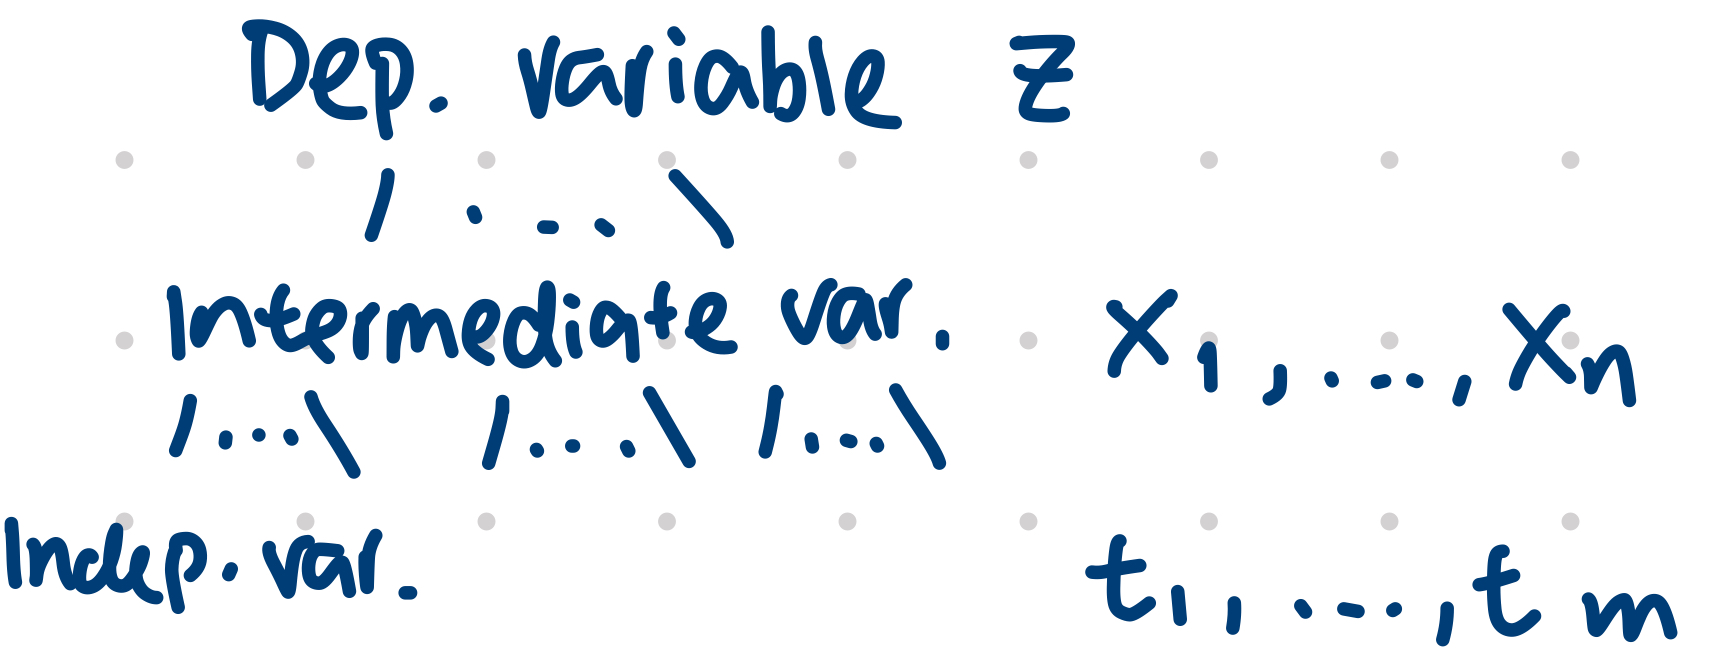
\includegraphics[scale=0.05]{chain-rule.jpg}

\begin{itemize}
    \item \keyword{Implicit Differentiation}{Given $F(x,y,z) = 0$, $z$ is implicitly defined by $x$ and $y$}
\end{itemize}
\[
    z_x = -\frac{F_x}{F_z} \quad z_y = -\frac{F_y}{F_z}
\]

\begin{itemize}
    \item \keyword{Directional Derivative}{$D_u f(x,y) = \langle f_x,f_y \rangle \cdot u$ where $u$ is a unit vector}
    \begin{itemize}
        \item Which direction yields min/max. directional derivative? Min: $-\nabla f$, Max: $\nabla f$
    \end{itemize}
\end{itemize}

\section{04. Gradient Vector}

\begin{itemize}
    \item \keyword{Gradient Vector}{$\nabla f(x,y) = \langle f_x, f_y \rangle$}
    \begin{itemize}
        \item $\nabla f(x_0,y_0)$ is normal to level curve $f(x,y)=k$ at $(x_0,y_0)$
        \item $\nabla f(x_0,y_0,z_0)$ is normal to level surface $f(x,y,z)=k$ at $(x_0,y_0,z_0)$
        \item Tangent plane to level surface: $\nabla f(x_0,y_0,z_0) \cdot \langle x-x_0,y-y_0,z-z_0 \rangle = 0$
    \end{itemize}
    \item \keyword{Extrema}{Point larger/smaller than surrounding points}
    \begin{itemize}
        \item $f$ has local min/max. at $(a,b)$ and $f_x (a,b)$, $f_y (a,b)$ exist $\rightarrow$ $f_x (a,b) = f_y (a,b) = 0$
        \begin{itemize}
            \item Converse: Not necessarily true (Saddle point)
        \end{itemize}
    \end{itemize}
    \item \keyword{Critical Point}{$(a,b)$ where $f_x (a,b) = f_y (a,b) = 0$}
    \item \keyword{Extreme Value Theorem}{$f(x,y)$ is continuous on closed and bounded set $D \subseteq \mathbb{R}^2 \rightarrow$ There exists absolute min/max.}
    \item To find absolute min/max.:
    \begin{enumerate}
        \item Find values of $f$ at critical points of $D$
        \item Find extreme values of $f$ on boundary of $D$
    \end{enumerate}
    \item \keyword{Lagrange Multiplier}{Find extrema of $f$ with constraint $g(x,y) = k$}
    \begin{itemize}
        \item Suppose min/max. of $f$ with constraint $g(x,y)=k$ occurs at $(x_0,y_0)$:
        \[
            \nabla f(x_0,y_0)=\lambda \nabla g(x_0,y_0)
        \]
        \item Suppose min/max. of $f$ with constraint $g(x,y,z)=k$ occurs at $(x_0,y_0,z_0)$:
        \[
            \nabla f(x_0,y_0,z_0)=\lambda \nabla g(x_0,y_0,z_0)
        \]
        \item If there are 2 constraints $g(x,y,z)=c_1$ and $h(x,y,z)=c_2$ (i.e. Curve), then $\nabla f = \lambda \nabla g + \mu \nabla h$
    \end{itemize}
\end{itemize}

\section{05. Double Integral}

\begin{itemize}
    \item \keyword{Fubini's Theorem}{$\int_{a}^{b} \int_{c}^{d} f dy dx = \int_{c}^{d} \int_{a}^{b} f dx dy$}
    \item Type I: If $D = \{(x,y):a \leq x \leq b, g_1(x) \leq y \leq g_2(x)\}$, then $\iint_D f dA = \int_{a}^{b} \int_{g_1(x)}^{g_2(x)} f dy dx$
    \item Type II: If $D = \{(x,y):c \leq y \leq d, h_1(y) \leq x \leq h_2(y)\}$, then $\iint_D f dA = \int_{c}^{d} \int_{h_1(y)}^{h_2(y)} f dx dy$
    \item Draw vertical/hor. arrows. Bounded area cannot split.
    \item $\iint_D f dA = \iint_{D_1} f dA + \cdots + \iint_{D_n} f dA$
    \item Area of plane region: $A(D) = \iint_D 1 dA$
    \item \keyword{Polar Coordinates}{$(r, \theta)$ where $r$ is distance from origin to point and $\theta$ is angle from positive $x$-axis}
    \begin{itemize}
        \item $x = r \cos \theta$ $\quad$ $y = r \sin \theta$ $\quad$ $r = \sqrt{x^2 + y^2}$
        \item $\theta = \tan^{-1} \frac{y}{x}$
    \end{itemize}
\end{itemize}
\[
    \iint_R f(x,y) dA = \int_{\alpha}^{\beta} \int_{a}^{b} f(r \cos \theta, r \sin \theta) \textcolor{red}{(r)} dr d\theta
\]

\section{06. Triple Integral}

\begin{itemize}
    \item Type I: If $E = \{(x,y,z):(x,y \in D, u_1(x,y) \leq z \leq u_2(x,y))\}$ where $D$ is projection of $E$ onto $xy$-plane, then $\iint_E f dV = \iint_D (\int_{u_1(x,y)}^{u_2(x,y)} f dz)dA$
    \item Type II: If $E = \{(x,y,z):(y,z \in D, u_1(y,z) \leq x \leq u_2(y,z))\}$ where $D$ is projection of $E$ onto $yz$-plane, then $\iint_E f dV = \iint_D (\int_{u_1(y,z)}^{u_2(y,z)} f dx)dA$
    \item Type III: If $E = \{(x,y,z):(x,z \in D, u_1(x,z) \leq y \leq u_2(x,z))\}$ where $D$ is projection of $E$ onto $xz$-plane, then $\iint_E f dV = \iint_D (\int_{u_1(x,z)}^{u_2(x,z)} f dy)dA$
    \item Volume of solid: $V = \iiint_E 1 dV$
    \item \keyword{Cylindrical Coordinates}{$(r,\theta,z)$ where $z$ is distance from $xy$-plane to $P$}
\end{itemize}
\[
    \iiint_E f(x,y,z) dV =  \int_{\alpha}^{\beta} \int_{h_1(\theta)}^{h_2(\theta)} \int_{u_1(r \cos \theta, r \sin \theta)}^{u_2(r \cos \theta, r \sin \theta)} 
\]
\[
    f(r \cos \theta, r\sin\theta,z)\textcolor{red}{(r)} dz dr d\theta
\]

\begin{itemize}
    \item \keyword{Spherical Coordinates}{$(\rho, \theta, \phi)$ where $\rho$ is distance from origin to $P$ and $\phi$ is angle from positive $z$-axis}
    \begin{itemize}
        \item $\rho \geq 0$ $\quad$ $0 \leq \theta \leq 2\pi$ $\quad$ $0 \leq \phi \leq \pi$
        \item $\rho^2 = x^2 + y^2 + z^2$ $\quad$ $x = \rho \sin \phi \cos \theta$
        \item $y = \rho \sin \phi \sin \theta$ $\quad$ $z = \rho \cos \phi$
        \item Good for spheres and cones
    \end{itemize}
\end{itemize}
\[
    \iiint_E f(x,y,z)dV = \int_{c}^{d} \int_{\alpha}^{\beta} \int_{a}^{b} 
\]
\[
    f(\rho \sin \phi \cos \theta, \rho \sin \phi \sin \theta, \rho \cos \phi)\textcolor{red}{(\rho^2 \sin \phi)} d\rho d\theta d\phi
\]

\section{07. Change of Variables}

\begin{itemize}
    \item \keyword{Plane Transformation}{$T: (u,v) \mapsto (x,y)$ given by $x=x(u,v)$ and $y=y(u,v)$}
    \begin{itemize}
        \item To get image $R$ under $T$, apply $T$ to boundary
    \end{itemize}
    \item \ilkeyword{Jacobian} of transformation $T$ given by $x=x(u,v)$ and $y=y(u,v)$:
    \[
        \partialderivative[(x,y)]{(u,v)} = \begin{vmatrix}
            \partialderivative[x]{u} & \partialderivative[x]{v} \\ 
            \partialderivative[y]{u} & \partialderivative[y]{v} \\ 
        \end{vmatrix}
        = \partialderivative[x]{u}\partialderivative[y]{v} - \partialderivative[x]{v}\partialderivative[y]{u}
    \]
    \item Change of Variable in Double Integral:
    \[
        \iint_{R} f(x,y) dA = \iint_{S} f(x(u,v),y(u,v)) \begin{vmatrix}\partialderivative[(x,y)]{(u,v)}\end{vmatrix} dudv
    \]
    \begin{itemize}
        \item $dA$ is image of rectangle $dudv$ under $T$
    \end{itemize}
    \item 3D:
    \[
        \partialderivative[(x,y,z)]{(u,v,w)} = \begin{vmatrix}
            \partialderivative[x]{u} & \partialderivative[x]{v} & \partialderivative[x]{w} \\ 
            \partialderivative[y]{u} & \partialderivative[y]{v} & \partialderivative[y]{w} \\ 
            \partialderivative[w]{u} & \partialderivative[w]{v} & \partialderivative[z]{w} \\ 
        \end{vmatrix}
    \]
    \[
        \iiint_{R} f(x,y,z) dA = \iiint_{S} f(x(u,v,w),
    \]
    \[
        y(u,v,w),z(u,v,w)) \begin{vmatrix}\partialderivative[(x,y,z)]{(u,v,w)}\end{vmatrix} dudvdw
    \]
    \item Tips:
    \begin{itemize}
        \item Choice of $T$ important! See from graph or integral
        \begin{itemize}
            \item Circle: $x=r\cos \theta$ and $y = r\sin \theta$
            \item Ellipse: $x=a r \cos \theta$ and $y = b r \sin \theta$
        \end{itemize}
        \item Find new bounds after $T$ and get Jacobian
        \item When finding Jacobian, if expressing $x,y$ with $u,v$ is difficult, can use $\partialderivative[(x,y)]{(u,v)} \partialderivative[(u,v)]{(x,y)} = 1$
    \end{itemize}
\end{itemize}

\section{08. Line Integral}

\begin{itemize}
    \item \keyword{Scalar Field}{Scalar function $f(x,y)$ or $f(x,y,z)$}
    \item \keyword{Vector Field}{Vector function $\mathbf{F}(x,y)$ or $\mathbf{F}(x,y,z)$}
    \begin{itemize}
        \item $\mathbf{F}(x,y,z) = \langle P(x,y,z),Q(x,y,z),R(x,y,z) \rangle$
    \end{itemize}
    \item\keyword{Line Integral over Scalar Field}{Suppose $C$ is parameterized by $\mathbf{r}(t) = \langle x(t),y(t) \rangle$ where $a \leq t \leq b$:}
    \[
        \int_{C} f(x,y) ds = \int_{a}^{b} f(x(t),y(t)) ||\mathbf{r}'(t)|| dt
    \]
    \begin{itemize}
        \item Intuition: Area of curtain above $C$ and under $f(x,y)$
        \item Independent of orientation
        \item Parameterization of line segment from $\mathbf{r}_0$ to $\mathbf{r}_1$: $\mathbf{r}(t) = \mathbf{r}_0 + (\mathbf{r}_1 - \mathbf{r}_0)t$ where $0 \leq t \leq 1$
        \item $\int_{C} f ds = \int_{C_1} fds + \cdots + \int_{C_n} fds$
        \item 3D: If $C$ is parameterized by $\mathbf{r}(t) = \langle x(t),y(t),z(t) \rangle$ where $a \leq t \leq b$, then $\int_C f(x,y,z)ds = \int_{a}^{b} f(x(t),y(t),z(t)) ||\mathbf{r}'(t)||dt$
    \end{itemize}
    \item \keyword{Line Integral of Vector Field}{Let $\mathbf{F}$ be continuous vector field defined on smooth curve $C$ parameterized by $\mathbf{r}(t) = \langle x(t),y(t),z(t) \rangle$ where $a \leq t \leq b$:}
    \[
        \int_C \mathbf{F} \cdot d\mathbf{r} = \int_C \mathbf{F} \cdot \mathbf{T} ds = \int_{a}^{b} \mathbf{F}(x(t),y(t),z(t)) \cdot \mathbf{r}'(t)dt
    \]
    \begin{itemize}
        \item Depends on orientation: $\int_{-C} \mathbf{F} \cdot d\mathbf{r} = -\int_{C} \mathbf{F} \cdot d\mathbf{r}$
        \item Check if parameterization has same orientation!
        \item Notation: $\int_{C} \mathbf{F} \cdot d\mathbf{r} = \int_{a}^{b} Px'(t)dt + \int_{a}^{b} Qy'(t)dt + \int_{a}^{b} Rz'(t)dt = \int_{a}^{b} Pdx + \int_{a}^{b} Qdy + \int_{a}^{b} Rdz$
    \end{itemize}
    \item \keyword{Conservative Vector Field}{Vector field $\mathbf{F}$ that can be written as $\mathbf{F} = \nabla f$ for some scalar function $f$}
    \begin{itemize}
        \item \keyword{Potential Function of $\mathbf{F}$}{$f$}
        \item Test for Conservative Field in 2D Plane: Suppose $\mathbf{F}(x,y)=\langle P,Q \rangle$ is a vector field in an \textbf{open and simply-connected} (i.e. No holes) region $D$ and both $P$ and $Q$ have continuous partial derivatives on $D$:
        \[
            \partialderivative[Q]{x} = \partialderivative[P]{y} \leftrightarrow \mathbf{F} \text{ is conservative on } D
        \]
        \item Test for Conservative Field in 3D Space: Suppose $\mathbf{F}(x,y,z)=\langle P,Q,R \rangle$ is a vector field in an \textbf{open and simply-connected} region $D$ and both $P$, $Q$, and $R$ have continuous partial derivatives on $D$:
        \[
            \partialderivative[Q]{x} = \partialderivative[P]{y}, \partialderivative[R]{x} = \partialderivative[P]{z}, \partialderivative[R]{y} = \partialderivative[Q]{z} 
        \]
        \[
            \leftrightarrow \mathbf{F} \text{ is conservative on } D
        \]
        \item If assumptions not met, cannot use these tests
    \end{itemize}
    \item \keyword{Fundamental Theorem for Line Integral}{Suppose $\mathbf{F}$ is a conservative vector field with potential function $f$ and $C$ is smooth curve from point $A$ to $B$:}
    \[
        \int_{C} \mathbf{F} \cdot d\mathbf{r} = \int_{C} \nabla f \cdot d\mathbf{r}= f(B) - f(A)
    \]
    \begin{itemize}
        \item $\exists$ 2 paths with same initial and terminal points with diff. line integrals $\rightarrow$ Vector field is not conservative
    \end{itemize}
    \item \keyword{Green's Theorem}{Let $C$ be \textbf{positively oriented}, piecewise-smooth, \textbf{simple closed} (i.e. No intersection with itself, except at start and end) and let $D$ be region bounded by $C$. Let $\mathbf{F}(x,y) = \langle P,Q \rangle$. If $P$ and $Q$ have continuous partial derivatives on open region with $D$:}
    \[
        \int_{C} \mathbf{F} \cdot d\mathbf{r} = \int_{C} Pdx + Qdy = \iint_{D} (\partialderivative[Q]{x} - \partialderivative[P]{y})dA
    \]
    \begin{itemize}
        \item Positive orientation: Counterclockwise
        \item $\partial D$: Positively oriented boundary of region $D$
        \item Area of Plane Region: Let $C$ be positively oriented, piecewise-smooth, simple closed curve in the plane and let $D$ be region bounded by $C$:
        \[
            A = \int_{C} xdy = -\int_{C} ydx = \frac{1}{2}(\int_{C} xdy - ydx)
        \]
    \end{itemize}
\end{itemize}

\section{09. Surface Integral}

\begin{itemize}
    \item \keyword{Parametric Surface}{Vector function $\mathbf{r}(u,v)=\langle x(u,v),y(u,v),z(u,v) \rangle$ parametrizes surface $S$ in $xyz$-space}
    \begin{itemize}
        \item How? $z = f(x,y)$, Cylindrical, Spherical Coord.
    \end{itemize}
    \item \keyword{Surface Integral of Scalar Field}{Let $S$ be parameterized by $\mathbf{r}(u,v) = \langle x(u,v),y(u,v),z(u,v) \rangle,(u,v) \in D$:}
    \[
        \iint_{S} f(x,y,z)dS 
    \]
    \[
        = \iint_{D} f(x(u,v),y(u,v),z(u,v))||\mathbf{r}_u \times \mathbf{r}_v||dA
    \]
    \begin{itemize}
        \item Tangent Plane of Surface: $\mathbf{r}_u (a,b) \times \mathbf{r}_v (a,b) \perp S$ at point $(x(a,b),y(a,b),z(a,b))$
        \item Special case: If $S$ is surface $z=g(x,y)$, then $\mathbf{r}_x \times \mathbf{r}_y=\langle -g_x, -g_y, 1 \rangle$ and:
        \[
            \iint_{S} f(x,y,z) dS 
        \]
        \[
            = \iint_{D} f(x,y,g(x,y)) (\sqrt{g_x^2 + g_y^2 + 1})dA
        \]
        \item Surface Area: $A(S) = \iint_{S} 1 dS = \iint_{D} ||\mathbf{r}_u \times \mathbf{r}_v|| dA$
    \end{itemize}
    \item \keyword{Oriented Surface}{Possible to define unit normal vector $\mathbf{n}$ at each point $(x,y,z)$ not on boundary such that $\mathbf{n}$ is continuous function of $(x,y,z)$}
    \begin{itemize}
        \item All orientable surfaces have 2 orientations
        \item \ilkeyword{Open Surface}
        \item \keyword{Closed Surface}{No boundary (e.g. Sphere, Donut)}
        \begin{itemize}
            \item Pos. orientation: Outward, Neg. orien.: Inward
        \end{itemize}
        \item $\mathbf{n} = \frac{\mathbf{r}_u \times \mathbf{r}_v}{||\mathbf{r}_u \times \mathbf{r}_v||}$ (Unit vec.) Opposite orientation: $-\mathbf{n}$
    \end{itemize}
    \item \keyword{Surface Integral of Vector Field}{(aka \ilkeyword{Flux} of $\mathbf{F}$ across $S$) Given 3D vector field $\mathbf{F}(x,y,z) = \langle P,Q,R \rangle$ and surface $S$ with given orientation $\mathbf{n}$:}
    \[
        \iint_{S} \mathbf{F} \cdot d\mathbf{S} = \iint_{S} \mathbf{F} \cdot \mathbf{n} dS = \iint_{D} \mathbf{F} \cdot (\mathbf{r}_u \times \mathbf{r}_v) dA
    \]
    \begin{itemize}
        \item Check orientation $\mathbf{n}$ of $S$ in qn. is given by $\frac{\mathbf{r}_u \times \mathbf{r}_v}{||\mathbf{r}_u \times \mathbf{r}_v||}$
        \item Special case: If $S$ is surface $z=g(x,y)$, then flux across $S$ in upward orientation:
        \[
            \iint_{S} \mathbf{F} \cdot d\mathbf{S} = \iint_{D} (-P g_x - Q g_y + R)dA
        \]
        \item Special case: Downward orientation
        \[
            \iint_{S} \mathbf{F} \cdot d\mathbf{S} = \iint_{D} (P g_x + Q g_y - R)dA
        \]
        \item Tips: Flat surfaces have constant $\mathbf{n}$, Not all components of $\mathbf{n}$ need to be computed, Plug in constraints when parameterizing $\mathbf{F}$ to simplify problem
        \begin{itemize}
            \item If using spherical coordinates ($r(\theta, \phi)$) to parametrize sphere of radius $\phi$: $r_\phi \times r_\theta = \langle \phi^2 \sin^2 \phi \cos \theta, \phi^2 \sin^2 \phi \sin \theta, \phi^2 \sin \phi \cos \phi \rangle$ (Outwards)
        \end{itemize}
    \end{itemize}
\end{itemize}

\section{10. Divergence and Curl}

\begin{itemize}
    \item \keyword{Divergence}{Scalar measure of net outflow of vector field}
    \begin{itemize}
        \item $\nabla = \langle \partialderivative[]{x},\partialderivative[]{y},\partialderivative[]{z} \rangle$
        \item 3D: $\text{div} F = \partialderivative[P]{x} + \partialderivative[Q]{y} + \partialderivative[R]{z} = \nabla \cdot F$
        \item 2D: $\text{div} F = \partialderivative[P]{x} + \partialderivative[Q]{y}$
    \end{itemize}
    \item \keyword{Gauss' Theorem}{Let $E$ be solid region where boundary surface $S$ is piecewise smooth with \textbf{positive} orientation. Let $F(x,y,z)$ be vector field whose component functions have \textbf{continuous partial derivatives} on an \textbf{open region} with $E$:}
\end{itemize}
\[
    \iint_{S} \mathbf{F} \cdot d\mathbf{S} = \iiint_E \text{div} \mathbf{F} dV
\]

\begin{itemize}
    \item \keyword{Curl}{Vector field measuring curling effect/circulation of underlying vector field}
    \begin{itemize}
        \item $\text{curl} F = \langle \partialderivative[R]{y} - \partialderivative[Q]{z},\partialderivative[P]{z} - \partialderivative[R]{x},\partialderivative[Q]{x} - \partialderivative[P]{y} \rangle = \nabla \times F$
        \item $\mathbf{F}$ is conservative $\rightarrow$ $\text{curl} \mathbf{F} = \text{curl} \nabla f = 0$
        \item $\text{div} (\text{curl} (\mathbf{F})) = 0$
    \end{itemize}
    \item \keyword{Stokes' Theorem}{Let $C$ be simple closed boundary curve of surface $S$ with unit normals $n$. Suppose that $C$ is \textbf{positively oriented with respect to $\mathbf{n}$}. Let $F$ be vector field whose components have continuous partial derivatives on open region that contains $S$:}
    \[
        \int_C \mathbf{F} \cdot d \mathbf{r} = \iint_S \text{curl} \mathbf{F} \cdot d \mathbf{S}
    \]
    \begin{itemize}
        \item Positively oriented with respect to $\mathbf{n}$: Right hand rule (Thumb follows $\mathbf{n}$)
        \item Stokes' Theorem is 3D version of Green's Theorem. Suppose $S$ is flat and lies in $xy$-plane with upward orientation $\mathbf{k}$:
        \[
            \int_C \mathbf{F} \cdot d \mathbf{r} = \iint_S \text{curl} \mathbf{F} \cdot \mathbf{k} dA = \iint_S \partialderivative[Q]{x} - \partialderivative[P]{y} dA
        \]
        \item If $S_1$ and $S_2$ are oriented surfaces with same oriented boundary curve $C$ and both satisfy assumptions of Stokes' Theorem: 
        \[
            \iint_{S_1} \text{curl} \mathbf{F} \cdot d\mathbf{S} = \int_{C} \mathbf{F} \cdot dr = \iint_{S_2} \text{curl} \mathbf{F} \cdot d\mathbf{S} 
        \]
        \item Flux of $\text{curl} \mathbf{F}$ over closed surface is 0
    \end{itemize}
\end{itemize}

\section{11. Others}

\begin{itemize}
    \item $\sin^2 \theta = \frac{1-\cos 2\theta}{2}$ $\quad$ $\cos^2 \theta = \frac{1+\cos 2\theta}{2}$
    \item $\int udv = uv - \int vdu$
\end{itemize}

\end{multicols*}
\end{document}
